The described geometries are simulated in CST Studio Suite and evaluated in the following. Simulation results include the electrical field, the magnetic field and the surface current distribution at \num{100} \si{\giga \hertz} and \num{1} \si{\tera \hertz}. Additionally, CST provides the radiation resistances of the antennas for different configurations. 

The distribution of the surface current is a measure of the electromagnetic wave's propagation through the antenna structure. Using the surface current distribution we can calculate the THz field emitted by the antenna using Maxwell's equations. Low frequency resonances caused by the large pad sizes are to be reduced. We present the surface current distribution in four H-Dipole antennas with differing NiCr-sections. The four configurations are compared at two distinct frequencies: \num{100} \si{\giga \hertz} (see figure \ref{sc_100ghz_comp}) and \num{1} \si{\tera \hertz}. The simulations at \num{100} \si{\giga \hertz} show that adding a NiCr-section to the antenna feed should reduce the low frequency surface current spikes caused by the antenna feeds and pads.


\begin{figure}[ht]
    \centering
    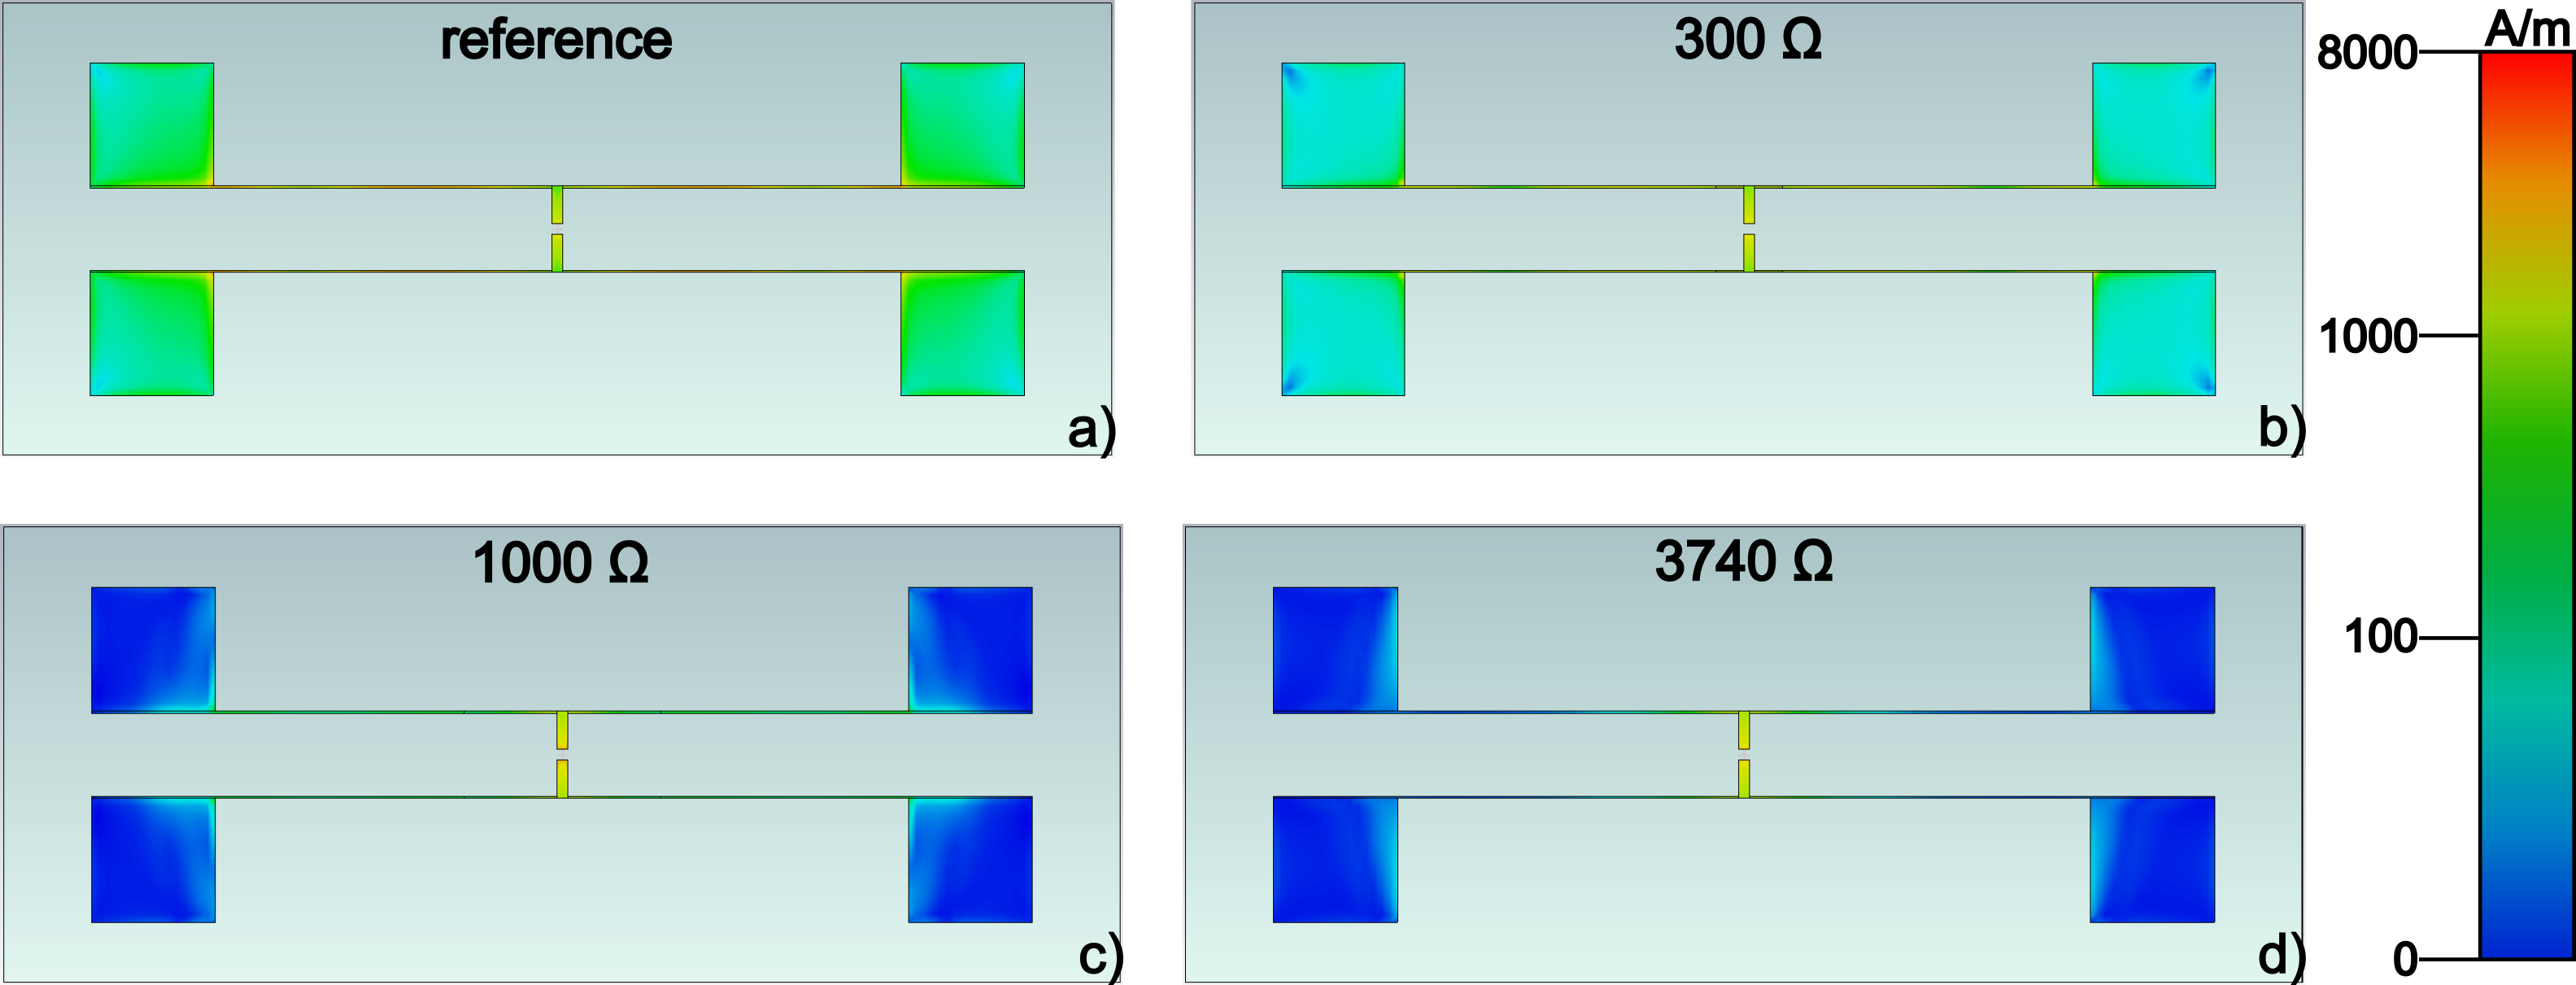
\includegraphics[width=\linewidth]{figures/Contour_Plots_v2/100Ghz_SC_sim_plots.png}
    \caption{Contour plots of the simulated surface currents at \num{100} \si{\giga \hertz} for four different H-Dipole antenna configurations. The surface current is plotted logarithmically. a) Surface current distribution in the reference H-Dipole. b) Surface current distribution with the NiCr-section corresponding to a resistance of $R_{NiCr} = 300$ \si{\ohm}. c) Surface current distribution with the NiCr-section corresponding to a resistance of $R_{NiCr} = 1000$ \si{\ohm}. d) Surface current distribution with the NiCr-section corresponding to a resistance of $R_{NiCr} = 3740$ \si{\ohm}.}
    \label{sc_100ghz_comp}
\end{figure}

Figure \ref{sc_100ghz_comp} a) depicts the surface current in the reference H-Dipole antenna where no NiCr is added. A fairly even distribution of the surface current along the antenna structure can be observed. Red sections along the antenna's feeding strip indicate that a high extend of the THz radiation is emitted in the strip, indicating the leaky-wave behavior of the antenna at low frequencies. Low-frequency harmonics are caused by these resonances along the feeding strip. We also see that the surface current distribution in the electrodes and the pads is fairly similar at surface currents of a few 100 A$/$m, causing the high low frequency resonances. 

A NiCr-section equivalent to a resistance of $R_{NiCr} = 300$ \si{\ohm} is added to the reference H-Dipole in figure \ref{sc_100ghz_comp} b). Already we can observe a concentration of the surface current around the antenna's electrodes. The surface current distribution in the pads now only reaches values of a few 10 A$/$m. Low frequency pad resonances still occur but are damped in a,amplitude. Along the feeding strips, resonant spots are observable, indicating that low frequency harmonics are still present. 


At $R_{NiCr} = 1000$ \si{\ohm} (see figure \ref{sc_100ghz_comp} c), the surface current is heavily concentrated around the antenna's electrodes. The surface current distribution in the pads nearly drops to zero. The surface current along the feeding strip appears relatively homogenous, indicating an absence of leaky-wave modes along the axis parallel to the strip and thus a reduction of low frequency time-harmonics. This is the non-resonant low frequency behavior we want to achieve. $R_{NiCr} = 3740$ \si{\ohm} (see figure \ref{sc_100ghz_comp} d)) is the maximum resistance we can achieve. A very similar surface current distribution compared to figure \ref{sc_100ghz_comp} c) is observable. The surface current along the feeding strip is further reduced and continues to concentrate around the electrodes. 

\begin{figure}[ht]
    \centering
    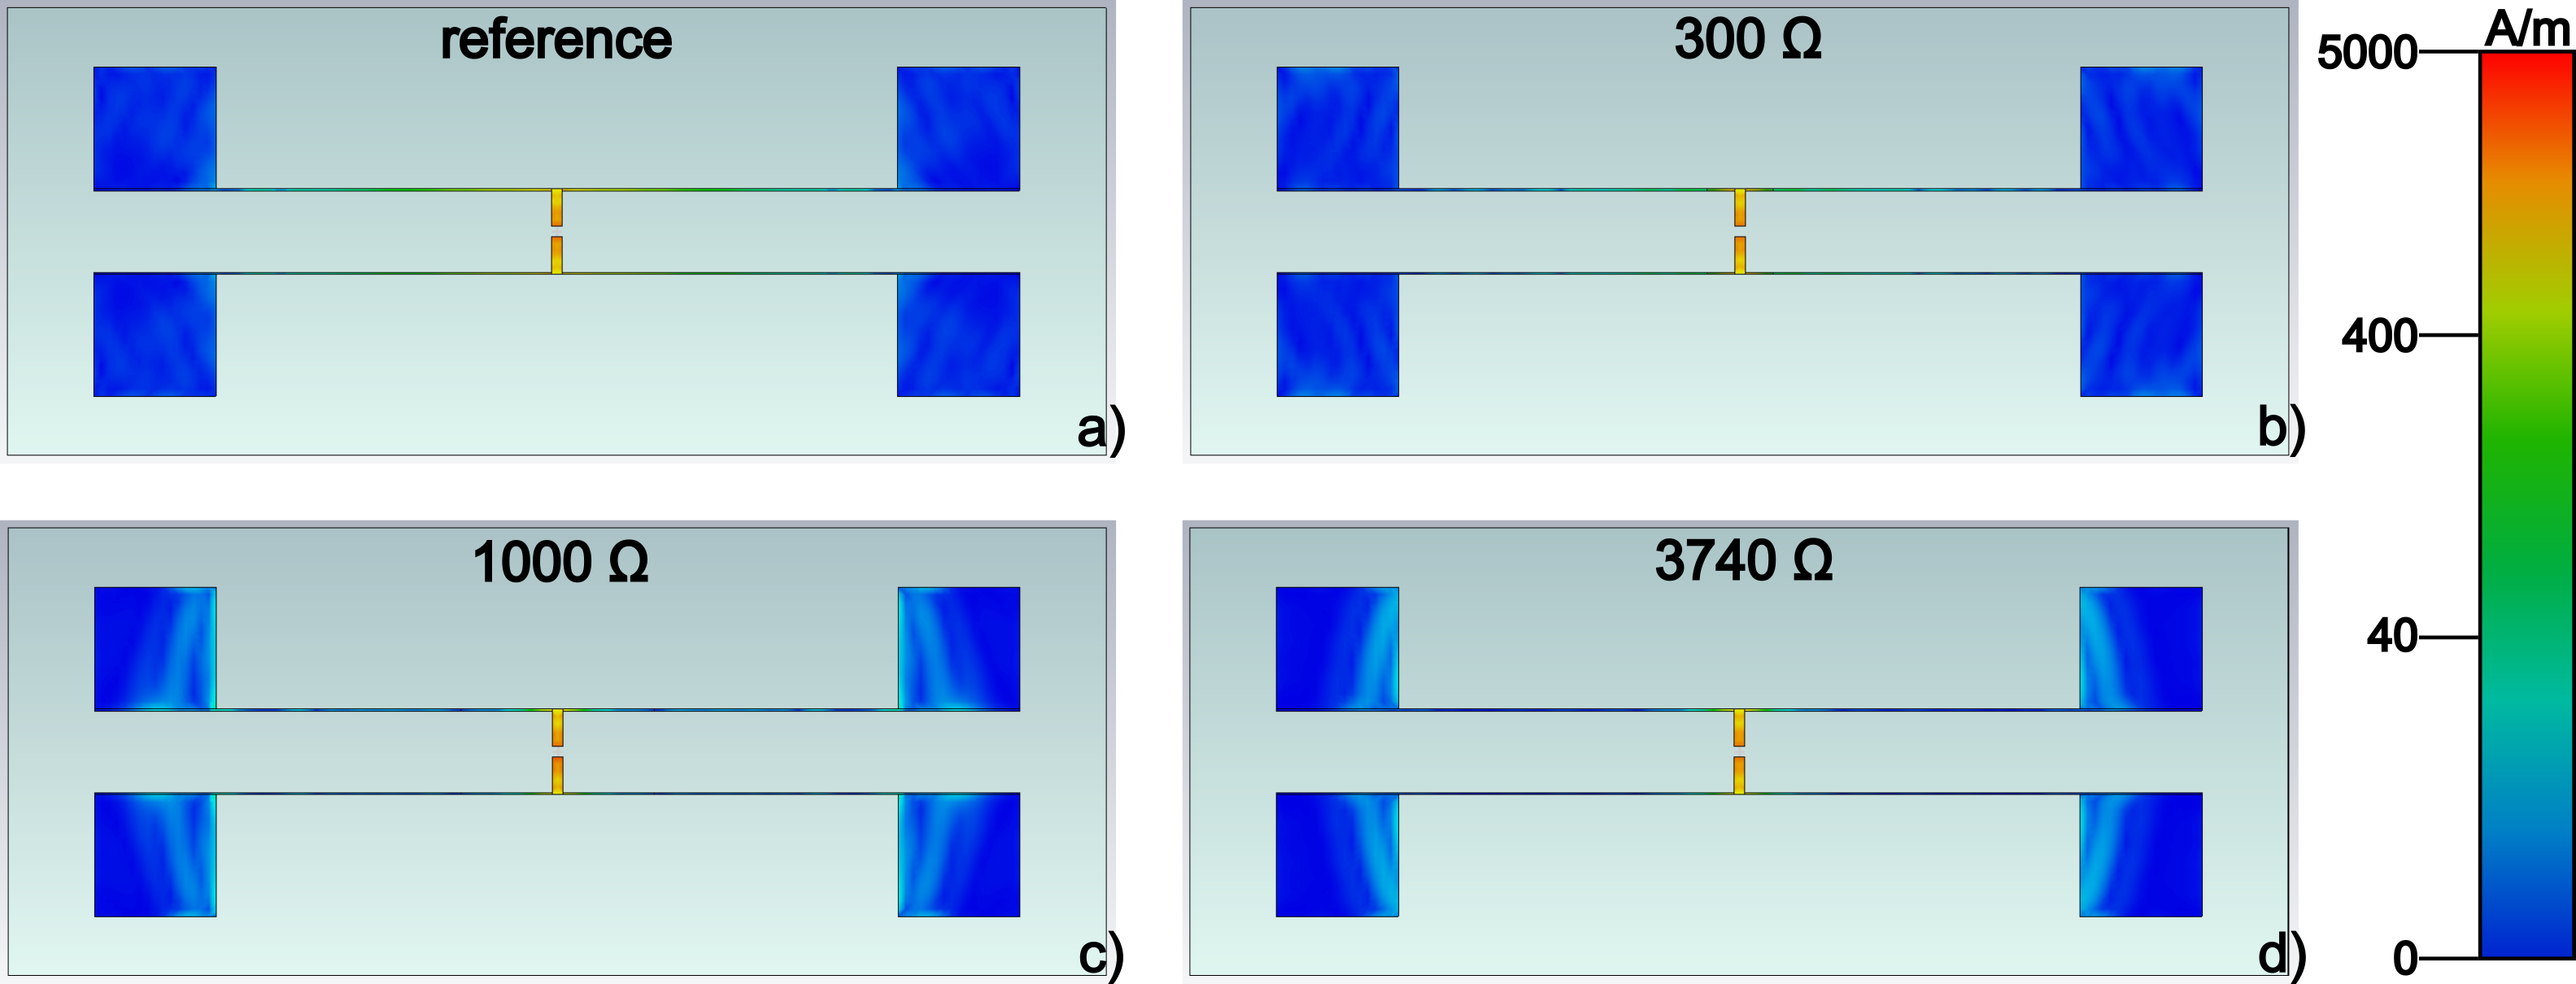
\includegraphics[width=\linewidth]{figures/Contour_Plots_v2/1Thz_SC_sim_plots.png}
    \caption{Contour plots of the simulated surface currents at \num{1} \si{\tera \hertz} for four different H-Dipole antenna configurations. The surface current is plotted logarithmically. a) Surface current distribution in the reference H-Dipole. b) Surface current distribution with the NiCr-section corresponding to a resistance of $R_{NiCr} = 300$ \si{\ohm}. c) Surface current distribution with the NiCr-section corresponding to a resistance of $R_{NiCr} = 1000$ \si{\ohm}. d) Surface current distribution with the NiCr-section corresponding to a resistance of $R_{NiCr} = 3740$ \si{\ohm}.}
    \label{sc_1thz_comp}
\end{figure}

It is important that adding the NiCr-section only affects the surface current generated at lower frequencies. At higher frequencies ($\nu > 100$ \si{\giga \hertz}), the coupling of THz radiation into the antenna is expected to occur predominantly at the electrodes due to the decreasing wavelength. Ideally, the NiCr segments should exert minimal influence on the surface currents propagating from the electrodes to the antenna pads. Figure \ref{sc_1thz_comp} shows the simulated surface current distribution at \num{1} \si{\tera \hertz} in the four antenna configurations which were already discussed at \num{100} \si{\giga \hertz}. 

At \num{1} \si{\tera \hertz}, the surface current distribution appears largely invariant across different antenna configurations. This antenna behavior is intended. The incorporation of NiCr segments introduces a resistive component that attenuates surface currents at lower frequencies. At higher frequencies, the surface current is able to propagate despite the added resistance. 



